\documentclass[10pt, a4paper,spanish]{article}

\usepackage[utf8]{inputenc}
\usepackage[spanish]{babel}

\usepackage[T1]{fontenc}

\usepackage[hmarginratio=1:1,top=32mm,columnsep=20pt]{geometry}
\usepackage[hang, small,labelfont=bf,up,textfont=it,up]{caption}

\usepackage{float}

\usepackage{amsmath}

\usepackage{enumitem}

\usepackage{graphicx}
\graphicspath{ {images/} }


\usepackage{titlesec}
\renewcommand\thesection{\Roman{section}}
\renewcommand\thesubsection{\Roman{subsection}}
\titleformat{\section}[block]{\large\scshape\centering}{\thesection.}{1em}{}
\titleformat{\subsection}[block]{\large}{\thesubsection.}{1em}{}

\usepackage{fancyhdr}
\pagestyle{fancy}
\fancyhead{}
\fancyfoot{}
\fancyhead[C]{ \today \ $\bullet$ Ingeniería del Conocimiento $\bullet$ Clips 2}
\fancyfoot[RO]{\thepage}

%-------------------------------------------------------------------------------
%	TITLE SECTION
%-------------------------------------------------------------------------------

\title{\vspace{-15mm}\fontsize{24pt}{10pt}\selectfont\textbf{Clips 2}} % Article title

\author{
	Fernández Angulo, Óscar \\
	\and
	García Prado, Sergio
}

\date{\today}

%-------------------------------------------------------------------------------

\begin{document}

	\maketitle % Insert title

	\thispagestyle{fancy} % All pages have headers and footers


%-------------------------------------------------------------------------------
%	TEXT
%-------------------------------------------------------------------------------

	\section{Sistema Cardiovascular Humano}

		\begin{enumerate}

			\item Cualquier desarreglo que afecta al corazón o a los vasos sanguíneos se considera una enfermedad cardiovascular. Así, un aneurisma (protuberancia) de la arteria abdominal, una estenosis arterial o la arteriosclerosis, que afectan a los vasos sanguíneos, son enfermedades cardiovasculares. La regurgitación aórtica, que ocurre cuando las válvulas de las aortas no son totalmente estancas, es una enfermedad cardiovascular que afecta al corazón.

			\item Así, cuando un paciente se queja de un dolor abdominal, una auscultación permite percibir un rumor abdominal y al palpar el abdomen del paciente se siente una masa pulsante, un aneurisma de la arteria abdominal probablemente cause estos síntomas y evidencias clínicas.

			\item Si la presión sistólica del paciente supera los 140 mmHg, la presión del pulso es superior a 50 mmHg, y al auscultar al paciente se percibe un rumor sistólico o una dilatación del corazón, todo ello puede estar causado por una regurgitación aórtica.

			\item Como último ejemplo, si un paciente siente calambres en las piernas al andar, que desaparecen tras uno o dos minutos de descanso, la presencia de una estenosis en una de las arterias de las piernas es más que probable. A su vez, la estenosis suele deberse a un problema de arteriosclerosis, especialmente si el paciente pertenece a algún grupo de riesgo: obeso o fumador durante más de 15 años o edad superior a 50 años.

		\end{enumerate}

		\paragraph{}
		La base de conocimiento necesaria para representar el problema requiere de un conjunto tanto de objetos como de atributos de los mismos. Esto se describe a continuación a partir de la Definición del Dominio (DD) y el conjunto de reglas:

		\begin{equation*}
			O = \{paciente, enfermedad, queja, riesgo \}
		\end{equation*}

		\begin{multline*}
			DA = \{ \\
				enfermedad.tipo^s, enfermedad.subtipo^s, enfermedad.lugar^s, \\
				paciente.edad^s:number, paciente.queja^m, \\
				paciente.sistolica^s:number, paciente.sistolica^s:number, paciente.pulso^s:number, \\
				paciente.auscultacion^m, paciente.riesgo^m \\
				queja.nombre^s, queja.duracion^s:number, queja.lugar^s\\
				riesgo.nombre^s, riesgo.duraccion^s:number\\
			\}
		\end{multline*}


		\begin{enumerate}[label={\textbf{R\theenumi:}}]

			\item
				\textbf{if} $equals(combustibleEnMotor, estado, f)$ \textbf{and} $equals(depositoCombustible, observacion, cero)$ \\
				\textbf{then} $add(depositoCombustible, estado, vacio)$ \textbf{fi}

		\end{enumerate}
		

		\begin{figure}[H]
			\begin{center}
				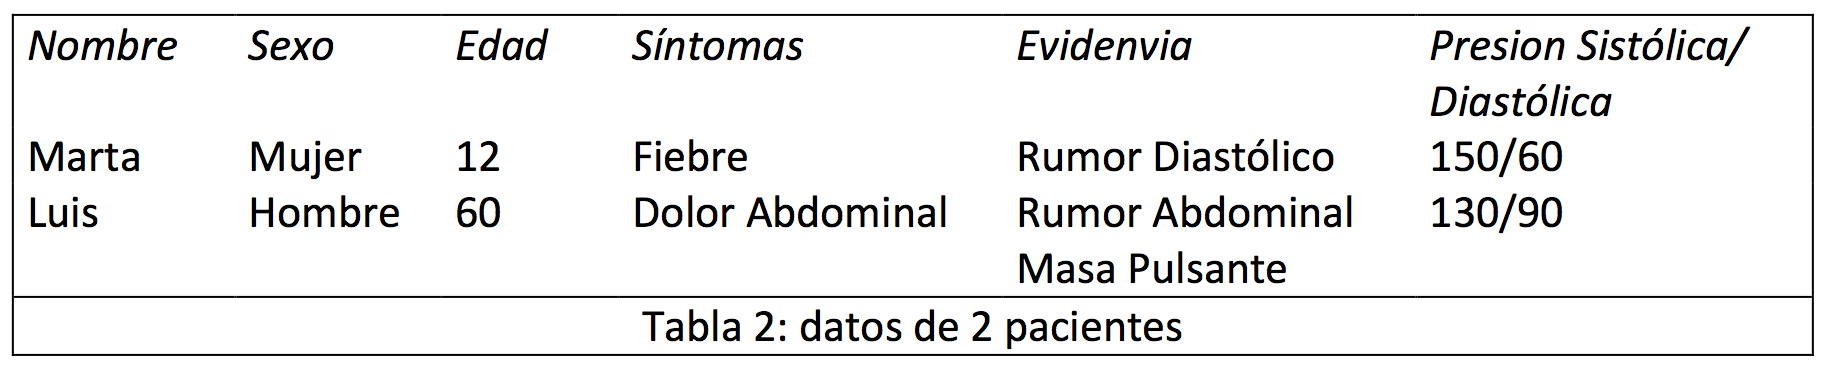
\includegraphics[width=0.75\textwidth]{table-2}
			\end{center}
		\end{figure}
\end{document}
